\chapter{Примери за използване}

\section{Пример за завършен анализ}

Най-естественият начин за използване на системата започва с качване на локално видео. Потребителят избира файл от файловата система, приложението го записва във файловото хранилище и създава съответен запис в таблицата \texttt{Videos}. От този момент нататък видеото става част от общата библиотека и може да бъде използвано като източник за нов анализ. Ако двата клиента работят върху една и съща конфигурация, записът става видим и в уеб, и в настолния интерфейс.

След като съществува качено видео, може да се създаде нов \texttt{AnalysisRun}. От гледна точка на потребителя това е кратко действие от интерфейса, но вътрешно то създава задача, която по-късно се поема от фоновия обработчик. Така потребителското действие се отделя от тежката аналитична обработка и системата остава отзивчива дори при по-дълги операции. След приключване на анализа в базата се записват статусът, резултатите от детекцията и обработеното видео.

След завършване на анализа потребителят може да прегледа подробностите за конкретно изпълнение. Тук системата показва използвания модел, броя на разпознатите обекти, обобщение по етикети, оригиналното видео, анотираното изходно видео и таблица с отделните detection results. По този начин приложението демонстрира завършен сценарий от качване на видео до преглед на финален резултат.

\begin{table}[htbp]
\centering
\begin{tabular}{ll}
\toprule
Показател & Стойност \\
\midrule
Изходно видео & \texttt{crowd.mp4} \\
Използван модел & \texttt{yolov8n.onnx} \\
Статус на анализа & \texttt{Completed} \\
Общо открити обекти & 424 \\
Основен клас & \texttt{person} -- 409 разпознавания \\
Други класове & \texttt{bird} -- 6, \texttt{dog} -- 5, \texttt{handbag} -- 2 \\
Допълнителни класове & \texttt{skis} -- 1, \texttt{suitcase} -- 1 \\
\bottomrule
\end{tabular}
\caption{Примерни стойности от завършен анализ на видео \texttt{crowd.mp4}}
\label{tab:crowd-analysis-results}
\end{table}

\cref{tab:crowd-analysis-results} показва реален резултат от изпълнение на анализа. В този пример системата разпознава голям брой хора в кадрите, което съответства на съдържанието на видеото. Същите данни се визуализират както в Blazor клиента, така и в Avalonia клиента, когато двете приложения използват една и съща база данни и едно и също файлово хранилище.

\begin{lstlisting}[caption={Съкратен лог от изпълнението и обновяването на анализа}, label={code:analysis-demo-log}, language={}]
Video uploaded: crowd.mp4
Analysis run created with model: yolov8n.onnx
Run status: Queued -> Processing -> Completed
Output video and detections are ready
Objects detected: 424
Top labels: person=409, bird=6, dog=5, handbag=2
\end{lstlisting}

Логът от \cref{code:analysis-demo-log} не е пълен системен журнал, а съкратено представяне на съществените състояния в процеса на обработка. Те показват преминаването от качено видео към чакаща задача, последваща обработка, завършен анализ и записани резултати. Така примерът описва реален процес на обработка, а не визуализация на статични примерни данни.

\section{Екрани за демонстрация}

Екраните в тази секция показват завършения сценарий в двата потребителски интерфейса и илюстрират, че резултатите от анализа се четат от общия приложен слой. Blazor изгледът представя най-пълната визуализация на анализа, докато Avalonia изгледът използва същите данни и същите ViewModel-и в настолен клиент.

\IfFileExists{figures/screenshots/blazor-analysis-details_1.png}{
    \begin{figure}[htbp]
        \centering
        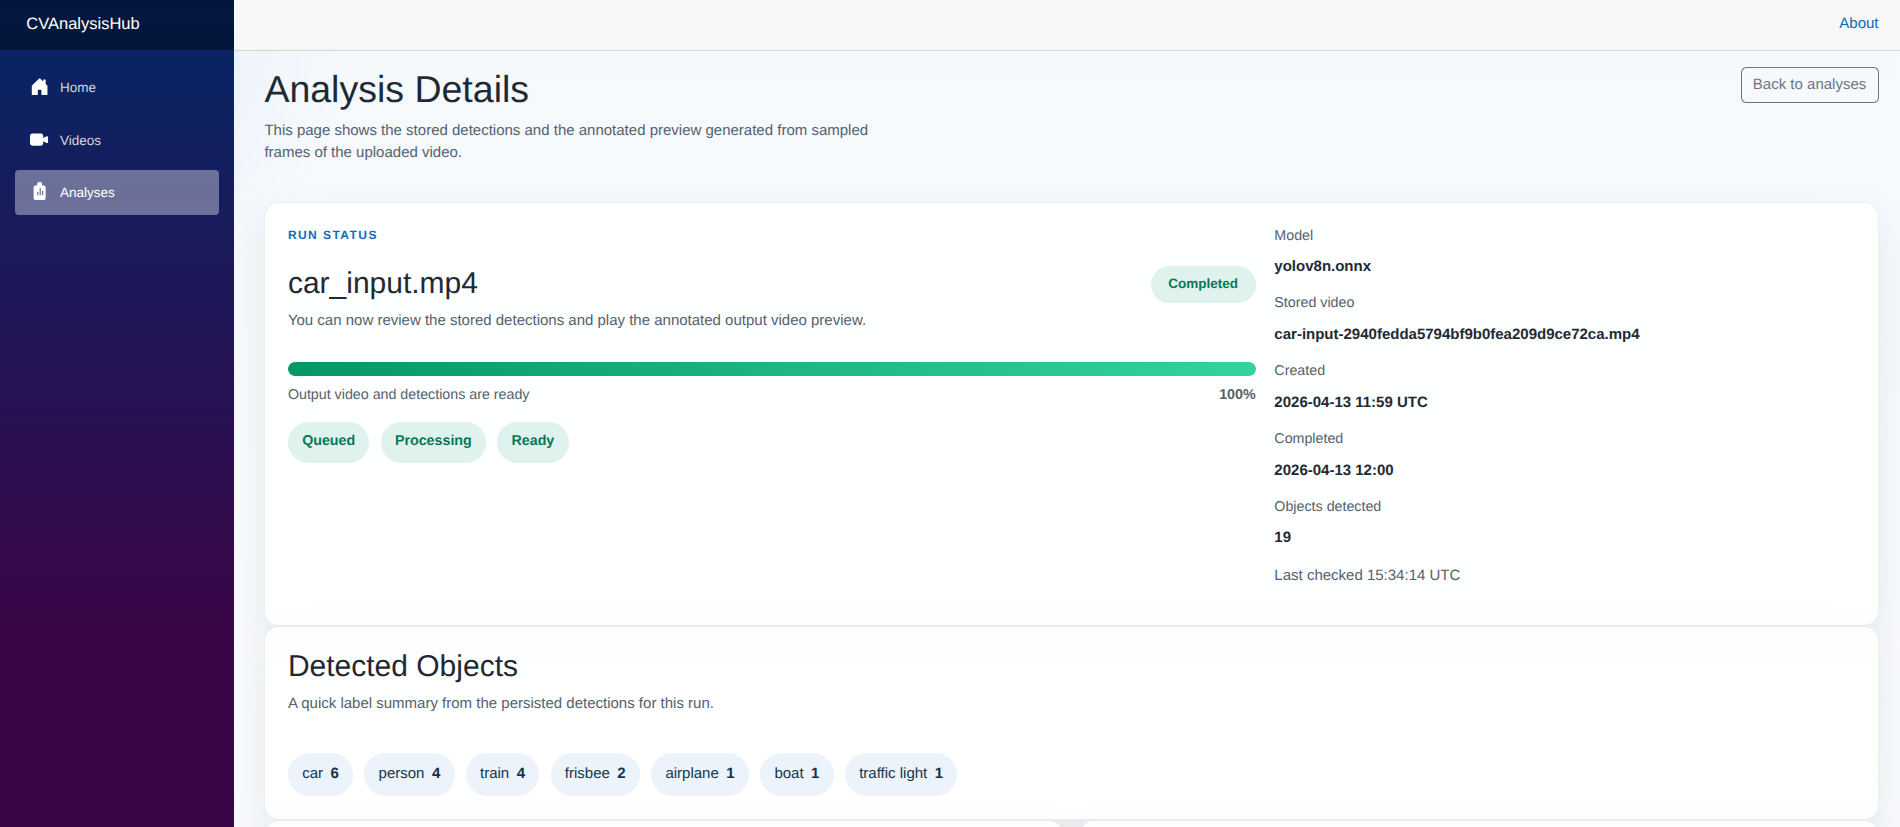
\includegraphics[width=0.95\textwidth,height=0.58\textheight,keepaspectratio]{figures/screenshots/blazor-analysis-details_1.png}
        \caption{Blazor интерфейс с подробности за завършен анализ, обобщение на разпознатите обекти и видео визуализация}
        \label{fig:blazor-analysis-details-overview}
    \end{figure}
}{}

\IfFileExists{figures/screenshots/blazor-analysis-details_2.png}{
    \begin{figure}[htbp]
        \centering
        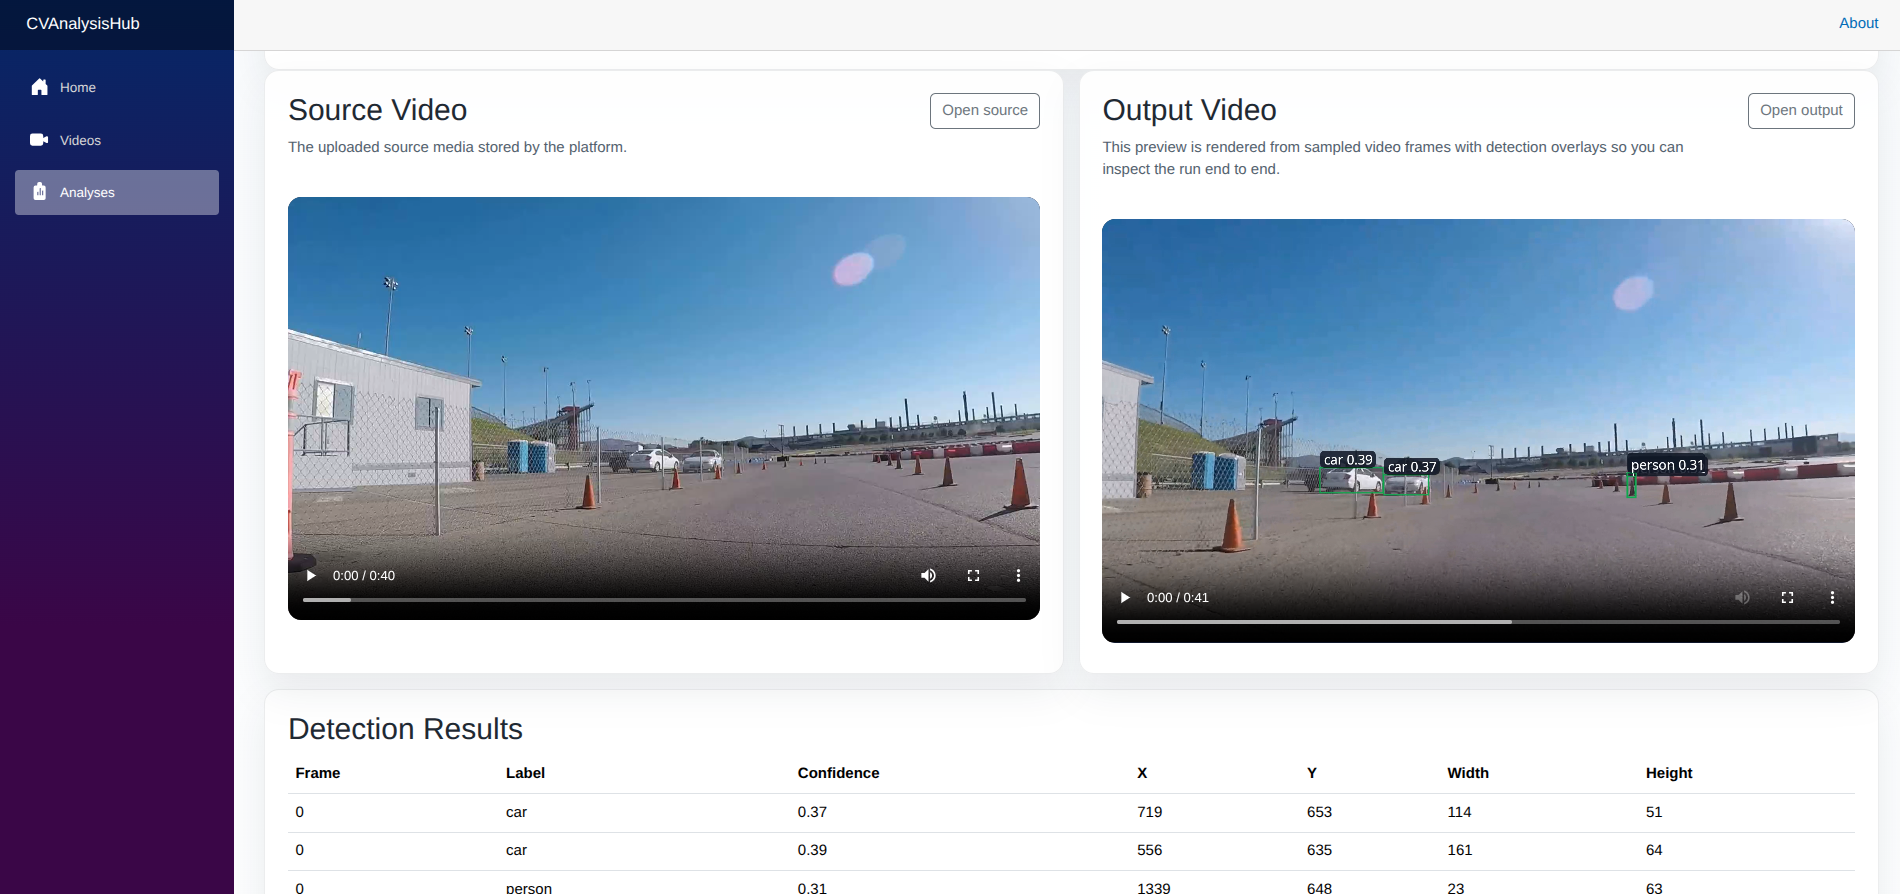
\includegraphics[width=0.95\textwidth,height=0.58\textheight,keepaspectratio]{figures/screenshots/blazor-analysis-details_2.png}
        \caption{Blazor интерфейс с таблица на отделните detection results за завършения анализ}
        \label{fig:blazor-analysis-details-results}
    \end{figure}
}{}

\IfFileExists{figures/screenshots/avalonia-analysis-details.png}{
    \begin{figure}[htbp]
        \centering
        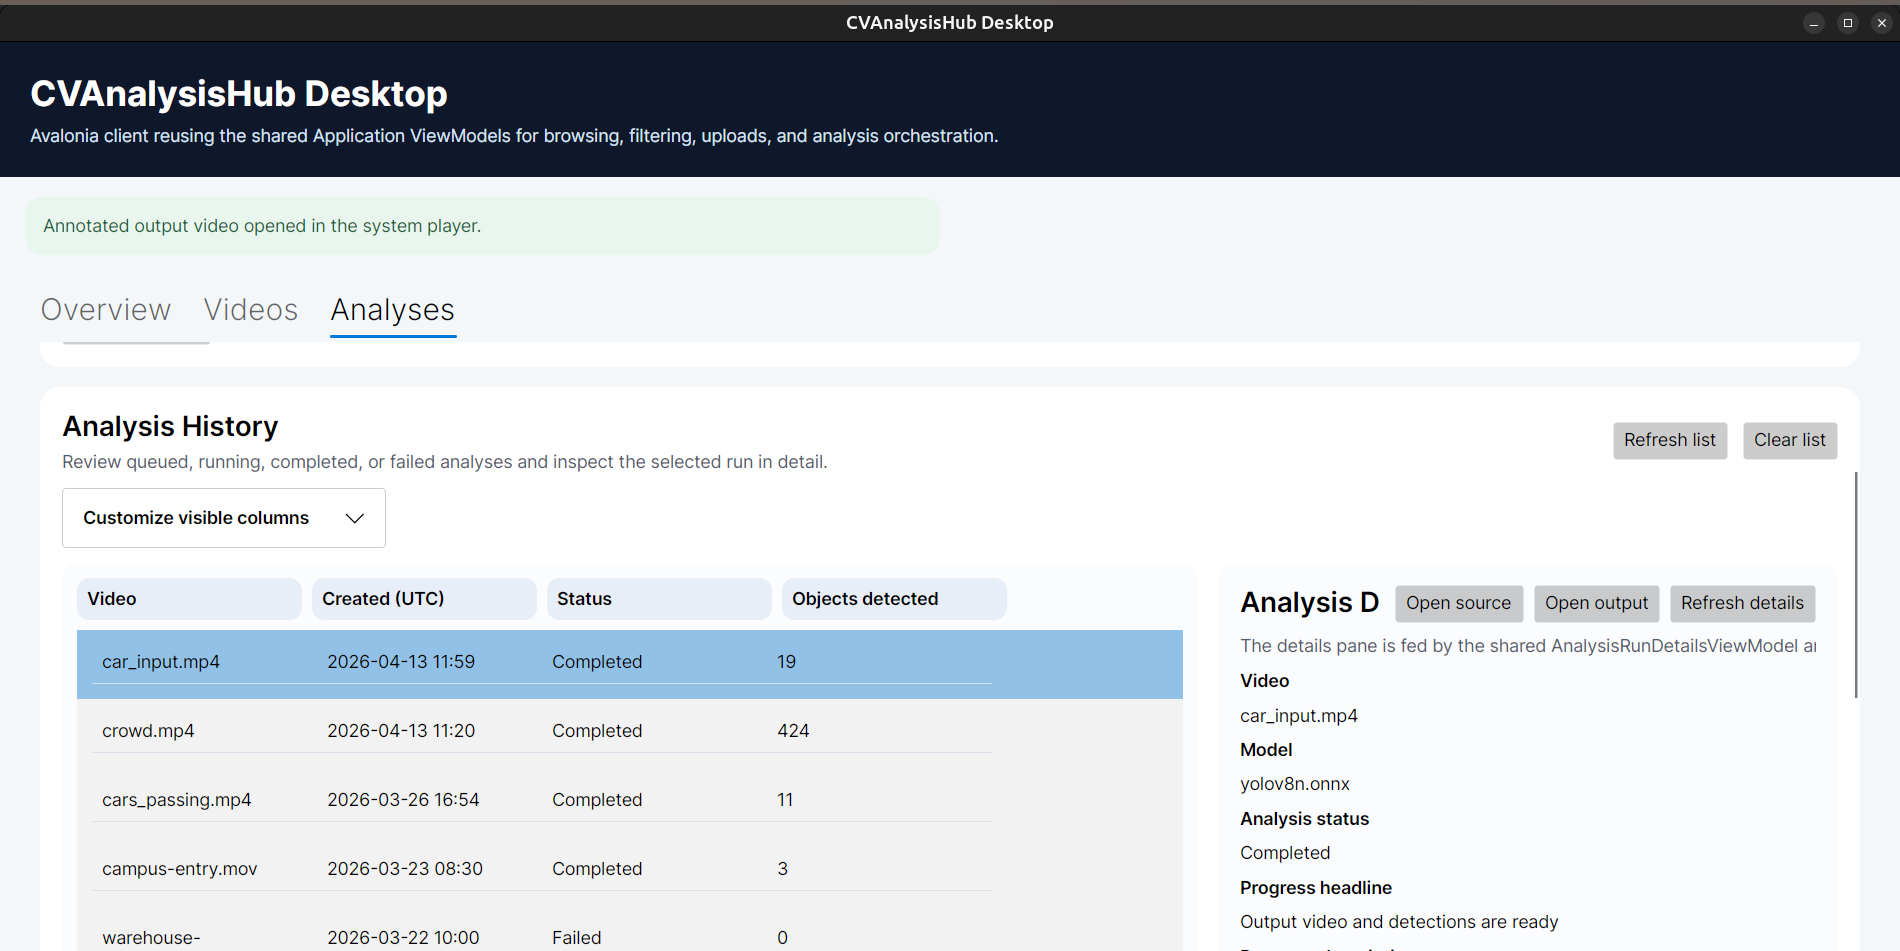
\includegraphics[width=0.95\textwidth,height=0.58\textheight,keepaspectratio]{figures/screenshots/avalonia-analysis-details.png}
        \caption{Avalonia интерфейс със същия завършен analysis run и синхронизирани резултати}
        \label{fig:avalonia-analysis-details}
    \end{figure}
}{}

\IfFileExists{figures/screenshots/reusable-filters-list.png}{
    \begin{figure}[htbp]
        \centering
        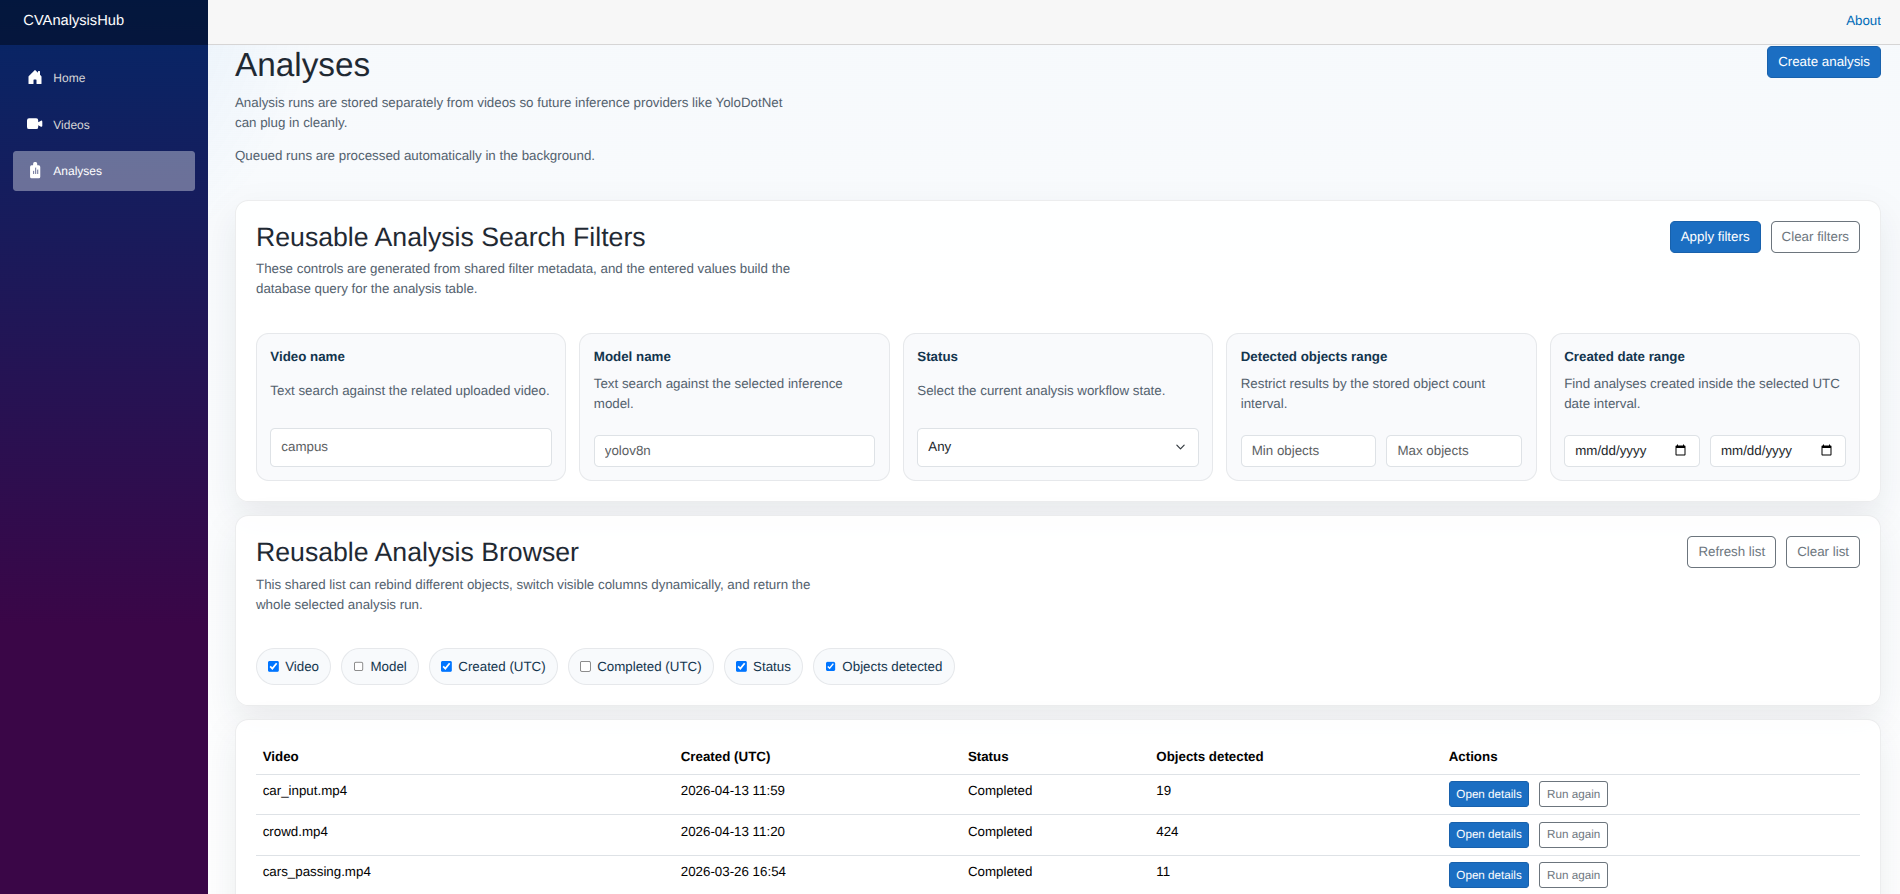
\includegraphics[width=0.95\textwidth,height=0.58\textheight,keepaspectratio]{figures/screenshots/reusable-filters-list.png}
        \caption{Демонстрация на преизползваемо филтриране и преизползваема визуализация на списък от обекти}
        \label{fig:reusable-filters-list}
    \end{figure}
}{}

\section{Демонстрация на преизползване}

Уеб клиентът показва преизползваемо филтриране върху два различни набора от данни. При \texttt{Videos} са реализирани филтри по име, статус, продължителност и дата на качване, а при \texttt{AnalysisRuns}, по видео, модел, статус, брой открити обекти и дата на създаване. Същественото е, че една и съща инфраструктура за филтриране работи върху различни модели без да бъде писана отново за всеки от тях.

Подобен ефект се наблюдава и при преизползваемата визуализация на списъци от обекти. Потребителят може да променя видимите колони, да избира конкретен ред и да работи с целия съответстващ обект, независимо каква част от него е визуализирана в таблицата. Тази функционалност е приложена както за \texttt{Videos}, така и за \texttt{AnalysisRuns}, което показва, че механизмът работи върху повече от един тип данни.
